\begin{figure}
    \centering
    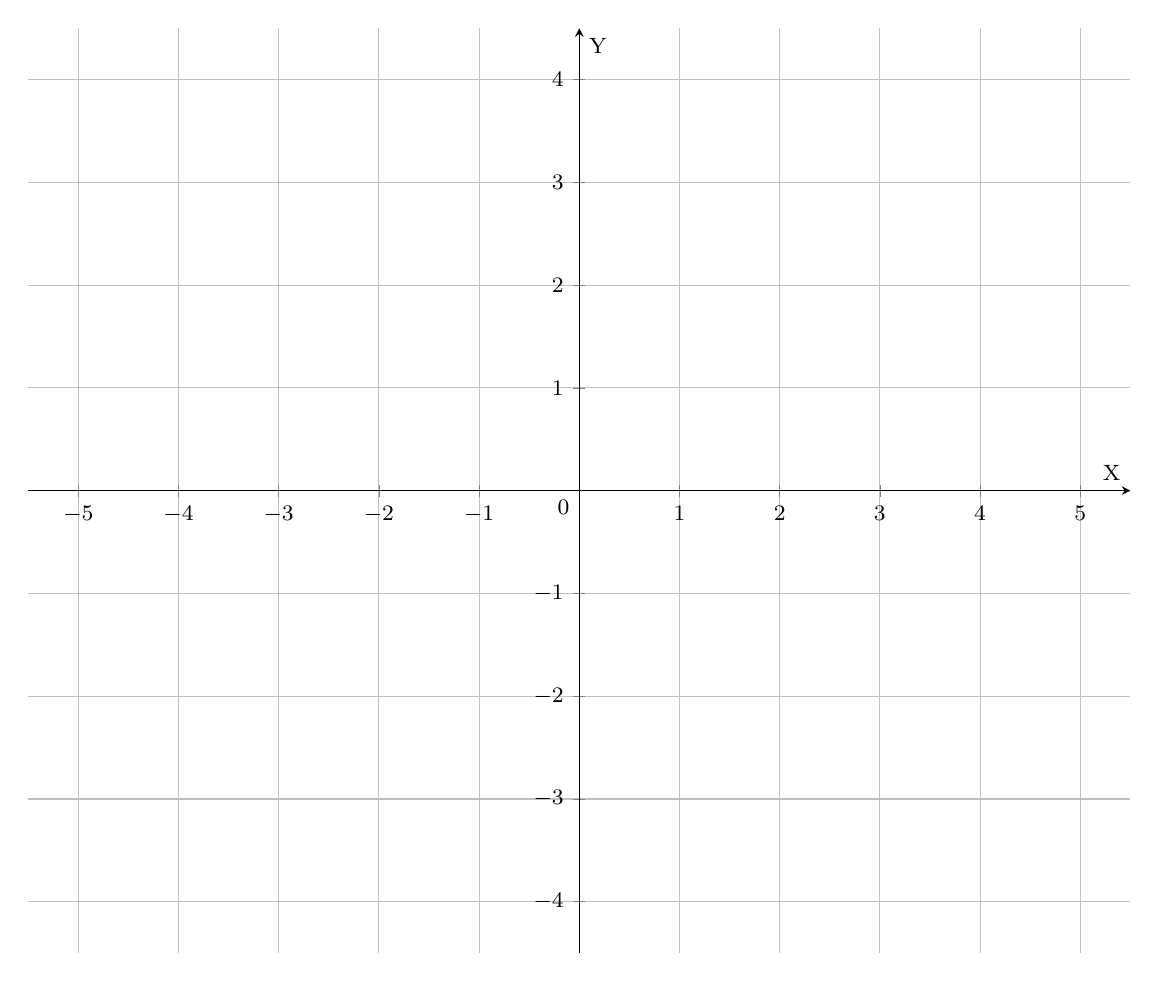
\begin{tikzpicture}
    \begin{axis}[scale=1.5,
                font=\footnotesize,
    	    width=.9\linewidth,
    		xlabel={X},ylabel={Y},
    		xtick = {-5,-4,...,5},
    		ytick = {-4,-3,...,4},
    		xmin=-5.5,xmax=5.5,
    		ymin=-4.5,ymax=4.5,
    		restrict y to domain=-5:5,
    		axis lines=center,
    		grid=both,
    		% grid style={line width=.1pt, draw=gray!10},
            % major grid style={line width=.2pt,draw=gray!50},
            % minor tick num=4,enlargelimits={abs=0.5},
    		% axis lines=center,
    % 		axis equal image,
    		]
    		
    		\node[below left] at (0,0) {$0$};
        	
        	% \addplot[domain=-pi:pi,samples=200,
% line width=1.5pt, blue] ({4*cos(deg(x))},{3*sin(deg(x))});
        	% \addplot[only marks,mark =*,blue,line width=2.5pt] coordinates{(-2,2) (10,2) (4,-2) (4,6)};
    	\end{axis}    
    \end{tikzpicture}
    % \caption{Caption}
    % \label{fig:my_label}
\end{figure}